% ============================================================
%  Minimum-Container Packing of a Non-Convex Polygon
%  via Simulated Annealing and Bracketing-Bisection Search
%
%  Graduate Report, Applied Mathematics and Numerical Methods
%  Joel Solis, University of Arizona
% ============================================================
\documentclass[10pt,twocolumn]{article}

\usepackage[margin=1.8cm,top=2.2cm,bottom=2.2cm]{geometry}
\usepackage{amsmath,amssymb,amsthm}
\usepackage{graphicx}
\usepackage{booktabs}
\usepackage[hidelinks]{hyperref}
\usepackage{microtype}
\usepackage[font=small,labelfont=bf]{caption}
\usepackage{algorithm}
\usepackage{algpseudocode}
\usepackage{enumitem}
\setlist{noitemsep,topsep=2pt}

\setlength{\columnsep}{18pt}
\setlength{\parskip}{3pt}
\setlength{\parindent}{10pt}

\newtheorem{remark}{Remark}

\title{%
  \textbf{Minimum-Container Packing of a Non-Convex Polygon\\
  via Simulated Annealing and Bracketing-Bisection Search}\\[4pt]
  {\normalsize Graduate Report, Applied Mathematics and Numerical Methods}%
}

\author{Joel Solis\\[2pt]
  {\small Department of Mathematics, University of Arizona}\\
  {\small\texttt{jsolis@math.arizona.edu}}%
}

\date{}

\begin{document}
\maketitle
\thispagestyle{empty}

% ============================================================
\begin{abstract}
A 2024 Kaggle competition posed a deceptively simple question: given
$N$ identical, irregular rigid pieces, how small a square can contain
them all without overlap? Answering this exactly is NP-hard.
This report describes a practical solver built around two-phase
Simulated Annealing (SA) guided by an outer bracketing-bisection loop
that certifiably narrows the interval containing the true minimum side
length $L^*$. Collision detection uses the Separating Axis Theorem (SAT),
a deliberate choice: SAT returns penetration depth, converting a
combinatorial feasibility problem into a differentiable energy function
the SA can navigate. We derive complexity estimates for the SA schedule
and collision kernel, analyze how temperature governs effective step size
and expected collision count, and report computational results for
$N \in \{5, 10, 25, 50, 100, 200\}$ across a five-node SLURM cluster
with 4 to 8 hours of wall time. Observed packing densities range from
$\eta \approx 0.58$ at small $N$ to $\eta \approx 0.48$ at $N = 200$,
with feasibility becoming substantially harder to achieve as $N$ grows.
\end{abstract}

% ============================================================
\section{Introduction}
\label{sec:intro}

The problem is easy to state. Take a fixed non-convex polygon, make
$N$ identical copies, and find the smallest square that can hold all
of them without overlap, each copy free to translate and rotate. As
$N$ grows, the configuration space expands exponentially and exact
enumeration becomes hopeless.

Even the restricted case where all pieces are unit disks is
NP-complete~\cite{demaine2007}, as feasibility of the placement decision
reduces to a variant of bin-packing. Non-convex polygons are harder
still: the Minkowski sum characterizing pairwise overlap between two
non-convex pieces is non-convex and potentially disconnected, so no
compact feasibility certificate exists.

The method of last resort for problems of this class is stochastic
local search. As Sokal observed: ``Monte Carlo is an extremely bad
method; it should be used only when all alternative methods are
worse.'' That is precisely the situation here. We use Simulated
Annealing, accept that it is slow and resource-intensive, and design
the surrounding infrastructure to extract the most from the available
compute budget.

Section~\ref{sec:related} reviews related approaches.
Section~\ref{sec:formulation} states the problem mathematically.
Section~\ref{sec:complexity} derives complexity and runtime estimates.
Section~\ref{sec:algorithm} develops the algorithm.
Sections~\ref{sec:experiments} and~\ref{sec:results} describe the
experimental setup and present results.

% ============================================================
\section{Related Work}
\label{sec:related}

Geometric packing appears throughout operations research, manufacturing
(sheet nesting), and combinatorial geometry. The literature divides
into exact methods, No-Fit Polygon heuristics, and metaheuristics.

\paragraph{Exact and NFP methods.}
The No-Fit Polygon (NFP) is the locus of positions at which one
polygon just touches but does not overlap another.
Bennell and Oliveira~\cite{bennell2008} survey how NFPs reduce
pairwise overlap detection to a Minkowski sum computation, giving an
exact characterization of the feasibility boundary. For convex polygons,
the NFP is convex and computed in $O(m_1 + m_2)$ time. For non-convex
polygons it is generally non-convex and possibly disconnected, requiring
convex decomposition~\cite{ghosh1993}. Because our polygon has genuine
concavities, NFP-based exact methods are impractical at the sizes
we consider.

\paragraph{Simulated annealing for packing.}
Leung et al.~\cite{leung2003} showed that penalty-based energy
functions for SA consistently outperform approaches restricted to
strictly feasible states: hard feasibility constraints fragment the
search space into disconnected islands, trapping local methods.
Continuous penalties create navigable bridges between those islands.
Jakobs~\cite{jakobs1996} found that warm-starting SA from a structured
initial placement substantially reduces time to feasibility.

\paragraph{Genetic and population-based approaches.}
Genetic algorithms (GAs) treat entire layouts as chromosomes and
combine them via crossover. Burke et al.~\cite{burke2006} showed that a
GA encoding placement sequences discovers structurally diverse
configurations simultaneously, something a single SA chain cannot do.
Defining meaningful crossover operators for continuous rigid-body
placements remains non-trivial, and per-generation cost scales with $N$
in a way that makes GAs expensive beyond $N = 100$.

\paragraph{Parallel tempering.}
Parallel Tempering (PT) runs multiple SA chains at different temperatures
and periodically proposes Metropolis swaps between adjacent
chains~\cite{hukushima1996,earl2005}. High-temperature chains explore
freely; cold chains refine. Hukushima and Nemoto established that PT
mixes exponentially faster than single-chain SA on multimodal
landscapes. The present implementation uses independent multi-start SA;
PT is a natural next step, though preliminary experiments under
one-hour budgets found no feasible solutions under the PT variant
tested, suggesting it requires substantially longer runs to benefit.

\paragraph{Position of this work.}
We adopt the penalty-energy reformulation of Leung et al., add a
three-level AABB hierarchy and SAT depth computation for collision
detection, and place SA inside an outer bracketing-bisection-polish
loop that provides a certified bound on $L^*$. The combination of
bisection-certified bounds with an adaptive long-run polish and
deterministic HPC-safe seeding has not, to our knowledge, been applied
to this specific non-convex problem.

% ============================================================
\section{Problem Formulation}
\label{sec:formulation}

Let $\mathcal{P}$ be a fixed polygon with 15 vertices and area
$A_p \approx 0.2456$ (by the shoelace formula). Placing the $i$-th copy
requires a centre $c_i = (x_i, y_i)$ and a rotation angle $\theta_i
\in [0, 2\pi)$. The world vertices are $w_k^{(i)} = R(\theta_i)v_k +
c_i$, where $\{v_k\}_{k=0}^{14}$ are the reference vertices and
$R(\theta)$ is the standard $2 \times 2$ rotation matrix.

A configuration is \emph{feasible} if no two copies overlap and every
copy lies within $\Omega_L = [-L/2,\,L/2]^2$. The optimization problem is
\begin{equation}
  L^* = \min\, L \quad \text{s.t.} \quad \exists\;
  \text{feasible config.\ of } N \text{ copies in } \Omega_L.
  \label{eq:opt}
\end{equation}

\paragraph{Area lower bound.}
The combined area of all copies must fit inside $\Omega_L$, giving the
hard lower bound
\begin{equation}
  L_{\mathrm{area}} = \sqrt{N A_p}.
  \label{eq:area_bound}
\end{equation}
Every candidate $L < L_{\mathrm{area}}$ is provably infeasible and is
skipped without any SA evaluation. For $N = 100$,
$L_{\mathrm{area}} \approx 4.956$.

\paragraph{Why strict feasibility enforcement fails.}
Restricting the search to non-overlapping configurations at all times
confines it to a union of disconnected feasible islands in
$\mathbb{R}^{2N} \times [0,2\pi)^N$. A local method started on any
one island cannot reach another without crossing infeasible territory.
Allowing temporary, penalized violations creates navigable paths between
islands and is the key that makes stochastic search tractable here.

% ============================================================
\section{Complexity Analysis and Runtime Estimates}
\label{sec:complexity}

The estimates in this section use the polygon's bounding radius
$r_{\mathrm{br}} = 0.80$, area $A_p = 0.2456$, and the fan
triangulation into 13 triangles. They serve both to justify design
choices and to predict the fraction of wall time spent in each phase.

\subsection{SA Iterations, Collision-Free}

Each SA trial runs Phase A (70{,}000 iterations) then Phase B
(35{,}000), totaling $M = 105{,}000$ per trial. Ignoring collision,
each iteration is $O(1)$: pick a polygon, generate a displacement,
apply the Metropolis criterion. The full bracket-plus-bisect phase
requires at most
\[
  (350 + 182) \times M
  \;=\; 532 \times 105{,}000
  \;\approx\; 5.6 \times 10^7
\]
iterations (35 bracket steps at 10 trials each, 26 bisection steps at
7 trials each). At one nanosecond per iteration, this is under one
minute. Collision detection, not arithmetic, is the bottleneck.

\subsection{Collision Detection Cost Per SA Move}

When polygon $k$ moves, only its interactions with grid neighbours
are recomputed. Let $\eta = NA_p/L^2$ be the packing density. The
grid cell size is $h = 2r_{\mathrm{br}} = 1.6$, and a search radius of
$R = 2$ covers a $5 \times 5$ block of 25 cells. The expected number of
neighbour polygons per query is
\begin{equation}
  k(\eta)
  \;=\; 25N\cdot\frac{h^2}{L^2}
  \;=\; \frac{100\,r_{\mathrm{br}}^2\,\eta}{A_p}
  \;\approx\; 261\eta.
  \label{eq:kneigh}
\end{equation}
At $\eta = 0.85$, about 222 candidate pairs are queried per move.
Almost all are rejected by the polygon-level AABB check: two bounding
boxes of radius $r_{\mathrm{br}}$ can only overlap if centres are
within $2r_{\mathrm{br}}$ in both $x$ and $y$, covering an area of
$2.56$ against the $64$ area units searched, a pass fraction of~4\%.
Of the 222 queries, roughly 9 proceed to triangle-level inspection.
For those 9 pairs, the SAT kernel (six axes, $\sim$20 operations each,
169 triangle-pair combinations in the worst case but pruned by AABB)
costs approximately 2{,}400 operations per pair. The total per-move cost is
\begin{equation}
  C_{\mathrm{move}}(\eta)
  \;\approx\; 222\times 4 \;+\; 9\times 2{,}400
  \;\approx\; 22{,}500 \;\text{flops.}
  \label{eq:movecost}
\end{equation}
On a single core at $10^9$ flops/s, each SA move takes 20 to 30
microseconds. The bracket-plus-bisect phase therefore costs roughly
$5.6 \times 10^7 \times 25\,\mu\mathrm{s} \approx 23$ minutes per
worker, leaving the majority of a four-hour job for the polish phase.

\subsection{Temperature, Step Size, and Effective Search Radius}
\label{sec:temp}

Step sizes $s_{xy}$ and $s_\theta$ are not fixed; they adapt every
1{,}500 iterations based on the current acceptance rate. When the
acceptance rate exceeds 55\%, step sizes grow by factor 1.12; below
25\%, they shrink by 0.88. At high temperature $T$, the Metropolis
criterion accepts most proposals including those creating shallow
overlaps, so acceptance stays high and step sizes expand toward the
ceiling $s_{xy,\max} = 2.0$. As $T$ falls, fewer overlap-inducing moves
are accepted, the acceptance rate drops, and step sizes contract toward
$s_{xy,\min} = 10^{-5}$. Temperature and effective search radius thus
co-decrease automatically.

The overlap depth tolerated at temperature $T$ follows from the
Metropolis acceptance probability $e^{-\lambda d^p/T}$ for a move
creating penetration depth $d$. Setting this equal to $1/e$ gives the
characteristic tolerance:
\begin{equation}
  d_{\mathrm{tol}}(T) \;=\; \bigl(T/\lambda\bigr)^{1/p}.
  \label{eq:dtol}
\end{equation}
For Phase A ($p=1$, $\lambda=100$), at the start $d_{\mathrm{tol}} =
0.003$ and at the end $d_{\mathrm{tol}} = 3\times 10^{-6}$. The
polygon has unit scale, so overlaps are tolerated only up to 0.3\% of
its extent even at the hottest point in Phase A. The search stays near
the boundary of the feasibility set, not deep inside infeasible space.

The effective diffusion coefficient in configuration space is
$D(T) \approx \tfrac{1}{2}\alpha_{\mathrm{target}}\,s_{xy}^*(T)^2$
with target acceptance $\alpha_{\mathrm{target}} \approx 0.4$.
Since $s_{xy}^*(T)$ grows with $T$, diffusion is fast at high
temperature (broad exploration) and slow at low temperature (local
refinement). Phase A covers the transition from global exploration to a
roughly converged placement; Phase B compresses the result into strict
feasibility.

\subsection{Expected Collision Count at Density $\eta$}
\label{sec:expected_collisions}

For two polygons placed uniformly at random in $\Omega_L$, the
probability of overlap is bounded by the exclusion area over total area:
\[
  P(\text{overlap})
  \;\leq\; \frac{4\pi r_{\mathrm{br}}^2\,\eta}{N A_p}.
\]
The expected number of overlapping pairs is therefore
\begin{equation}
  \mathbb{E}[n_{\mathrm{ov}}]
  \;\leq\; \frac{2(N-1)\pi r_{\mathrm{br}}^2\,\eta}{A_p}.
  \label{eq:expected_ov}
\end{equation}
At $N=100$ and $\eta=0.85$, equation~\eqref{eq:expected_ov} gives
$\mathbb{E}[n_{\mathrm{ov}}] \lesssim 1{,}387$, an upper bound using
bounding circles rather than the true polygon geometry. In practice, at
temperature $T$ with penalty $\lambda$ the equilibrium total overlap
energy satisfies $E \sim T$ (Gibbs equipartition), so mean total depth
$\sum d_i \sim T/\lambda \to 0$ as $T \to 0$. The algorithm drives
collisions to zero as it cools.

\subsection{Bisection Convergence}

After $k$ bisection steps from an initial bracket of width
$\Delta L_0$, the residual uncertainty in $L^*$ is
$\Delta L_0/2^k$. With $k = 26$, this is
$\Delta L_0/2^{26} \approx 1.5\times 10^{-8}\,\Delta L_0$.
For a typical initial bracket of width 0.25, absolute precision reaches
$3.7\times 10^{-9}$. In practice the limit is the quality of SA
feasibility detection at each probe, not bisection arithmetic.

% ============================================================
\section{Algorithm}
\label{sec:algorithm}

\subsection{Collision Detection}

The polygon decomposes offline into a fan of 13 triangles from
vertex~0, grouped into three clusters of sizes $(5,5,3)$ to enable a
three-level AABB hierarchy.

\paragraph{Level 1: bounding circle and polygon AABB.}
For each candidate pair from the spatial grid, a distance-squared
check against $(2r_{\mathrm{br}})^2$ runs first, then a polygon-level
AABB check requiring four comparisons. Together these eliminate
roughly 96\% of candidate pairs before any triangle geometry is examined.

\paragraph{Level 2: group and triangle AABB.}
Surviving pairs proceed to group-level AABB checks (nine group-pair
comparisons) and then per-triangle AABB checks. Both use only interval
arithmetic on precomputed boxes, with no trigonometry.

\paragraph{Level 3: SAT with penetration depth.}
SAT is applied only when the AABB levels cannot rule out contact. For
two triangles $A$ and $B$, SAT projects both onto the six edge-normal
axes (three per triangle) and tests for a separating gap. If no gap
exists, the triangles overlap and the minimum overlap width across
all axes is the penetration depth $d > 0$.

This depth is what makes the energy approach work. A binary overlap
test would assign equal penalty to a barely-touching pair and a deeply
embedded one, giving a flat energy surface with no gradient for SA to
follow. The depth $d$ is a continuous geometric signal, larger when
configurations are worse, and feeding $d^p$ into the energy creates the
directional cue that guides the algorithm toward feasibility.

\subsection{Energy Function}

The total energy of a configuration at container size $L$ is
\begin{equation}
  E \;=\; \lambda\!\sum_{i<j}\sum_{(a,b)\in\mathcal{T}_{ij}}
  d(a,b)^{p}
  \;+\; \mu\sum_{i}\phi_i(L),
  \label{eq:energy}
\end{equation}
where $d(a,b)$ is the SAT penetration depth between triangles $a$
and $b$, and $\phi_i(L)$ is the squared boundary violation for copy $i$.
The exponent $p$ switches from 1 in Phase A to 2 in Phase B, making the
penalty stiffer near feasibility. The weights $\lambda$ and $\mu$ ramp
upward during Phase B (factor 1.8 every 1{,}200 iterations, capped at
$10^8$) to prevent the chain from settling into jammed configurations.

\subsection{Simulated Annealing Schedule}

Each trial runs two phases. Phase A is the exploration phase: high
starting temperature $T_0 = 0.30$, large steps, and linear overlap
penalty ($p=1$) allow pieces to relocate broadly across the square.
Phase B is the enforcement phase: temperature drops from 0.06 to
$10^{-6}$, penalty weights ramp, and steps shrink, compressing the
layout into strict feasibility.

\begin{table}[t]
\centering
\small
\caption{Two-phase SA schedule parameters.}
\label{tab:phases}
\setlength{\tabcolsep}{4pt}
\begin{tabular}{lcc}
\toprule
Parameter & Phase A & Phase B \\
\midrule
Iterations            & 70{,}000        & 35{,}000 \\
$T_{\mathrm{start}}$  & $3\times10^{-1}$& $6\times10^{-2}$ \\
$T_{\mathrm{end}}$    & $3\times10^{-4}$& $10^{-6}$        \\
$\lambda_0,\,\mu_0$   & $10^{2}$ (fixed)& $10^{3}$ (ramped)\\
Overlap power $p$     & 1               & 2 \\
Reinsertion prob.     & 2\%             & 0.5\% \\
Adapt window          & \multicolumn{2}{c}{1{,}500 iterations} \\
\bottomrule
\end{tabular}
\end{table}

Temperature decreases geometrically: $T_k = T_0\beta^k$ with
$\beta = (T_{\mathrm{end}}/T_{\mathrm{start}})^{1/M}$. Geometric
cooling allocates equal logarithmic time to each temperature decade,
empirically balancing exploration and convergence better than linear
schedules~\cite{Hajek1988}.

Each move selects a random polygon and either applies a small
translation with optional rotation (probability $1-p_{\mathrm{ri}}$)
or teleports the polygon to a uniform random position within $\Omega_L$
(probability $p_{\mathrm{ri}}$). Rare teleportation prevents the SA
from freezing in configurations where no small perturbation helps.
Energy changes are computed incrementally: only pairs involving the
moved polygon are recomputed via the spatial grid.

A reheating mechanism activates when the acceptance rate falls below
2\%: temperature is multiplied by 1.5 and capped at $2T_0$, preventing
premature freezing in Phase A.

\subsection{Outer Search: Bracketing, Bisection, and Polish}
\label{sec:outer}

\paragraph{Bracketing.}
Starting from a grid layout with 15\% padding, the algorithm shrinks
$L$ by 3\% or grows it by 5\% per step until both a feasible upper
bracket $L_{\mathrm{high}}$ and an infeasible lower bracket
$L_{\mathrm{low}} \geq L_{\mathrm{area}}$ are established.

\paragraph{Bisection.}
With the bracket established, 26 steps of binary search evaluate
$L_{\mathrm{mid}} = (L_{\mathrm{low}} + L_{\mathrm{high}})/2$. Before
each SA run at a new $L$, polygon centres are rescaled by
$\gamma = (L_{\mathrm{new}}/L_{\mathrm{old}})\times 0.98$. This
warm-start step preserves structural information from the prior feasible
arrangement, reducing the time to reach feasibility at the new $L$.

\paragraph{Polish.}
After bisection, the algorithm runs until wall time expires, attempting
$L \leftarrow L^*(1-\varepsilon)$ and updating $L^*$ on success. The
shrink step $\varepsilon$ adapts over windows of 20 attempts to target
a 35\% success rate, staying within $[10^{-5},\,2\times 10^{-3}]$.
Every improvement is written to disk immediately, and a global snapshot
is flushed on \texttt{SIGTERM}, so SLURM preemption loses no progress.

\begin{algorithm}[H]
\caption{Outer minimisation loop}
\label{alg:outer}
\small
\begin{algorithmic}[1]
\State Initialise $L$ from grid layout;\; $L_{\mathrm{low}}
       \leftarrow L_{\mathrm{area}}$
\State \textbf{Bracket:} shrink or grow $L$ by trial until feasible
       $L_{\mathrm{high}}$ and infeasible $L_{\mathrm{low}}$ are found
\State \textbf{Bisect:} 26 steps, warm-start positions at midpoint,
       update bracket
\State \textbf{Polish:} loop until wall time; adapt $\varepsilon$
       to maintain 35\% improvement rate
\end{algorithmic}
\end{algorithm}

\paragraph{Parallel execution.}
Each SLURM worker is a fully independent process. Its seed is derived
deterministically from (base seed, run ID, trial index) via SplitMix64
hashing, guaranteeing reproducibility without time-based reseeding.
Workers share no runtime state; the global best is found by a
post-hoc pass over all output CSV files.

% ============================================================
\section{Experimental Setup}
\label{sec:experiments}

All experiments ran on the University of Arizona HPC cluster under
SLURM. Two parallel launching strategies were used.

\paragraph{Five-node embarrassingly parallel jobs.}
Each main job allocated five exclusive nodes. One controller process
per node spawned as many workers as available CPUs permitted after
reserving a fixed number of cores for the OS (RESERVE\_CPUS). With the
default setting of 64 runs per node, up to 320 independent seeds ran
concurrently per job. Each worker wrote its own history log and
best-geometry CSV independently; no inter-worker communication occurred
during the run.

\paragraph{Single-node array jobs.}
A complementary set of SLURM array jobs ran one independent seed per
array task with at most two concurrent tasks per node. Array sizes
were $N=25$ (8 tasks), $N=50$ (6 tasks), $N=100$ (4 tasks), and
$N=200$ (2 tasks).

\paragraph{Smoke tests.}
Validation runs for $N=5$ and $N=10$ used a 3-minute wall time on
the five-node configuration. Their purpose was to verify the pipeline
end-to-end and obtain fast reference densities at small $N$ before
committing to multi-hour allocations.

\paragraph{Wall time and SA schedule.}
Jobs for $N \in \{25, 50, 100\}$ received 4 hours; the $N=200$ job
received 8 hours. The SA schedule (Table~\ref{tab:phases}) was not
modified across instance sizes. At $N=200$ each polygon therefore
receives on average $M/N = 525$ move proposals per trial versus
4{,}200 at $N=25$. The multi-start strategy partially compensates: with
many independent seeds running simultaneously, the probability that at
least one finds a good arrangement increases, even if any single chain
under-explores.

Bracketing used $K_b = 10$ SA trials per candidate $L$; bisection
used $K_b = 7$; polish used $K_p = 5$.

% ============================================================
\section{Results}
\label{sec:results}

\subsection{Quantitative Summary}

Table~\ref{tab:results} reports the best feasible side length $L^*$
found by the combined pool of workers for each $N$, together with the
packing efficiency $\eta = NA_p/(L^*)^2$. The area lower bound
$L_{\mathrm{area}}$ is given for reference. A packing with $\eta = 1$
would have zero interstitial space, which is geometrically impossible
for this shape; values above 0.90 are considered excellent for
non-convex polygons~\cite{leung2003}.

\begin{table}[h]
\centering
\small
\caption{Best feasible side length and packing efficiency by instance
size. $L_{\mathrm{area}} = \sqrt{N \cdot 0.2456}$ is the area lower
bound. Smoke-test runs ($N=5,10$) used 3 min wall time; all others
used 4 or 8 h. ``Runs feasible'' counts individual workers that found
at least one feasible configuration.}
\label{tab:results}
\setlength{\tabcolsep}{4pt}
\begin{tabular}{rcccccc}
\toprule
$N$ & $L_{\mathrm{area}}$ & $L^*$ & $\eta$ &
Runs feas. & $t_{\text{first}}$ (s) & Wall \\
\midrule
   5 & 1.108 & 1.472 & 0.567 & 15 &  5 & 3\,min \\
  10 & 1.568 & 2.056 & 0.581 & 15 &  6 & 3\,min \\
  25 & 2.478 & 3.315 & 0.559 &  6 &  8 & 4\,h \\
  50 & 3.504 & 4.652 & 0.567 &  4 & 46 & 4\,h \\
 100 & 4.956 & 6.785 & 0.533 &  3 & 53 & 4\,h \\
 200 & 7.009 & 10.104& 0.481 &  1 & 19 & 8\,h \\
\bottomrule
\end{tabular}
\end{table}

Three observations stand out. First, the number of workers reaching
feasibility drops sharply with $N$: from 15 of 15 smoke-test runs at
$N=5$ and $N=10$, to 6 at $N=25$, and to a single run at $N=200$.
This is consistent with the exponential growth in configuration space
and with the under-exploration expected when $M/N$ move proposals per
polygon per trial become insufficient. Second, the best-of-best density
$\eta$ decreases with $N$, from 0.58 at small $N$ to 0.48 at $N=200$,
suggesting that our fixed SA budget does not fully exploit the
concavities of the polygon at large scale. Third, the time to final
best is very long at $N = 50$ and $N = 100$ (medians of 3{,}657 and
3{,}254 seconds respectively), indicating that most improvement
comes from the polish phase rather than from bisection.

\subsection{Time-Series Analysis}

Figure~\ref{fig:timeseries} shows the evolution of the best known $L^*$
over wall time for the legacy instance sizes
$N \in \{5,10,25,50,100,200\}$, with one row per $N$. Each row shows
individual feasible traces per worker (thin lines) together with the
aggregate best-so-far envelope (thick line).

\begin{figure*}[t]
  \centering
  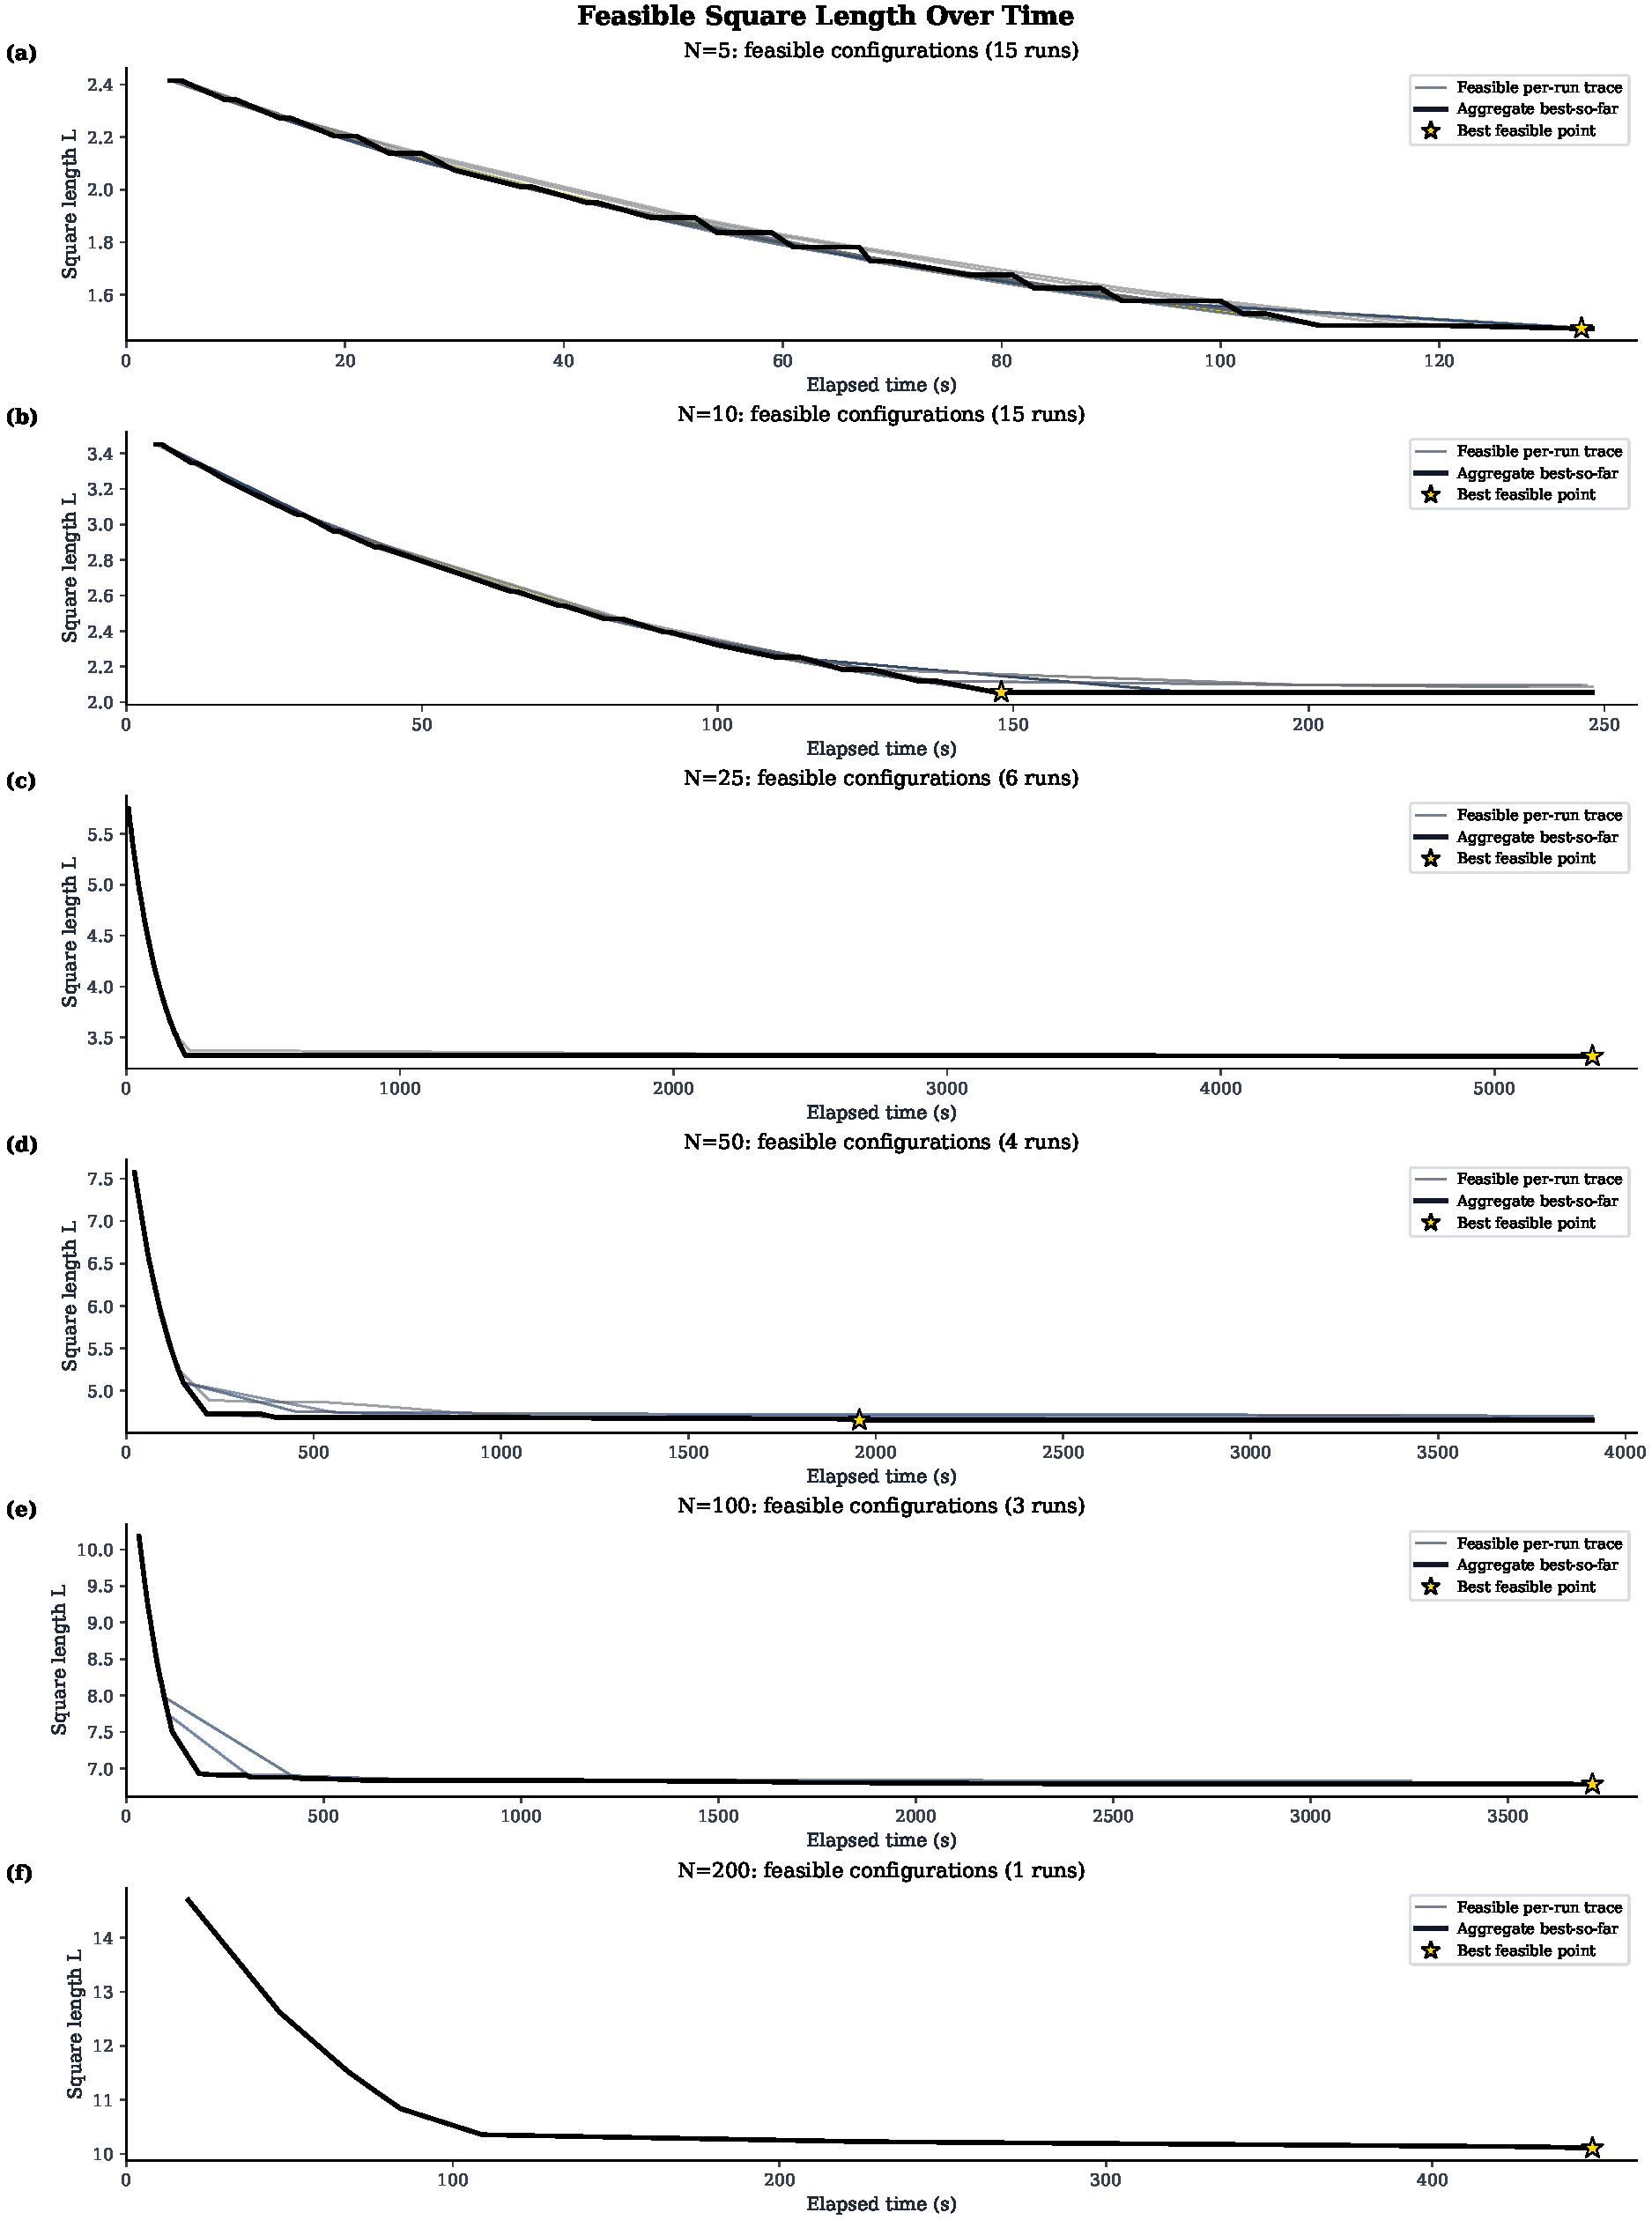
\includegraphics[width=\linewidth]{img/feasible_L_timeseries_rows_only_N5_N10_N25_N50_N100_N200}
  \caption{Feasible square length versus wall time for
  $N=5,10,25,50,100,200$, shown as rows of time-series only (no
  configuration inset column).}
  \label{fig:timeseries}
\end{figure*}

Figure~\ref{fig:pernconfigs} separates geometry from dynamics by
showing the best recovered packing configuration for each $N$ in its
own panel.

\begin{figure*}[t]
  \centering
  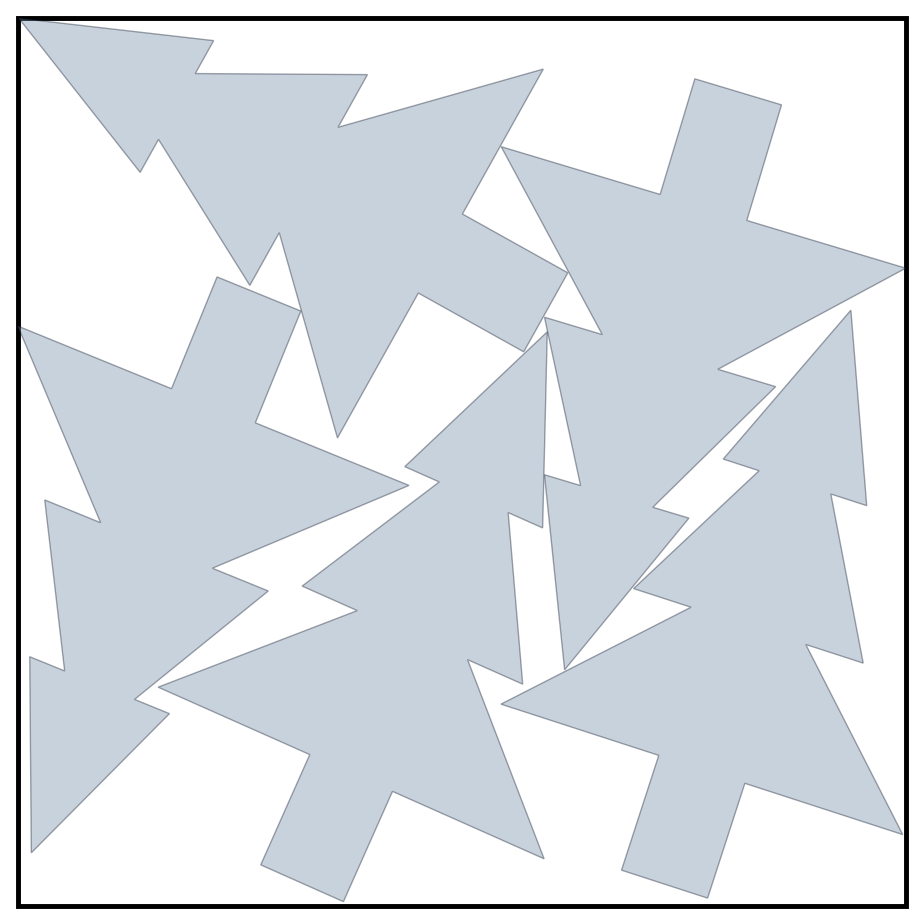
\includegraphics[width=0.32\linewidth]{img/per_n_configs/N005_best_config}\hfill
  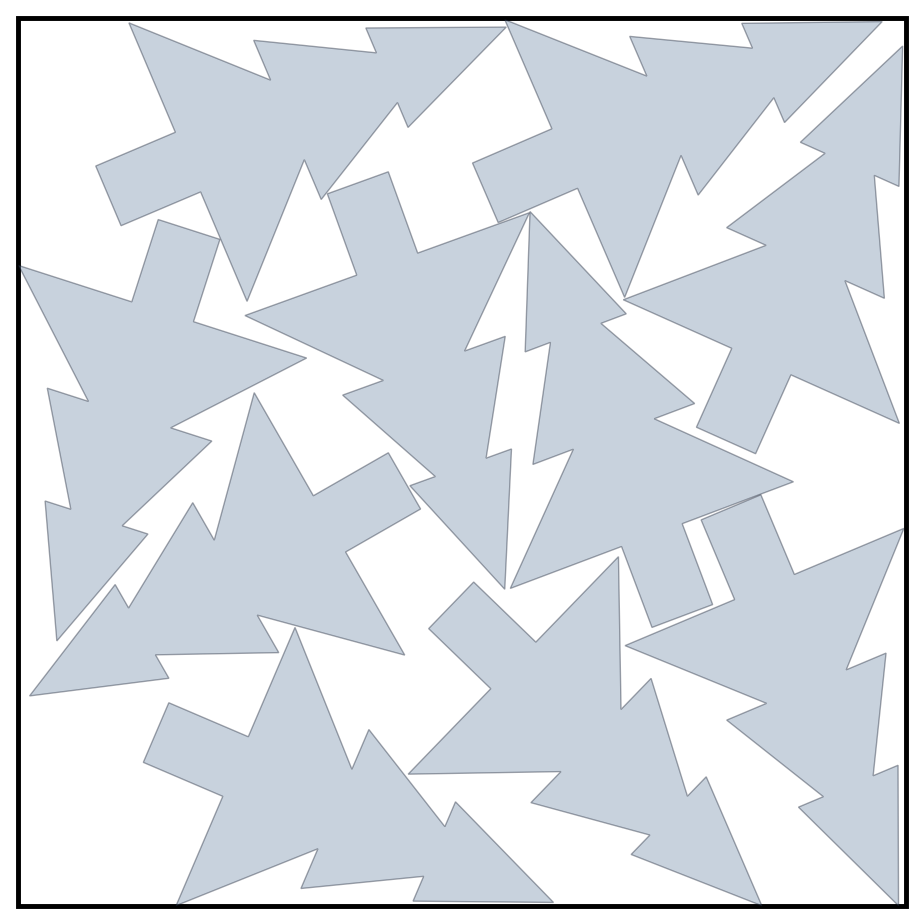
\includegraphics[width=0.32\linewidth]{img/per_n_configs/N010_best_config}\hfill
  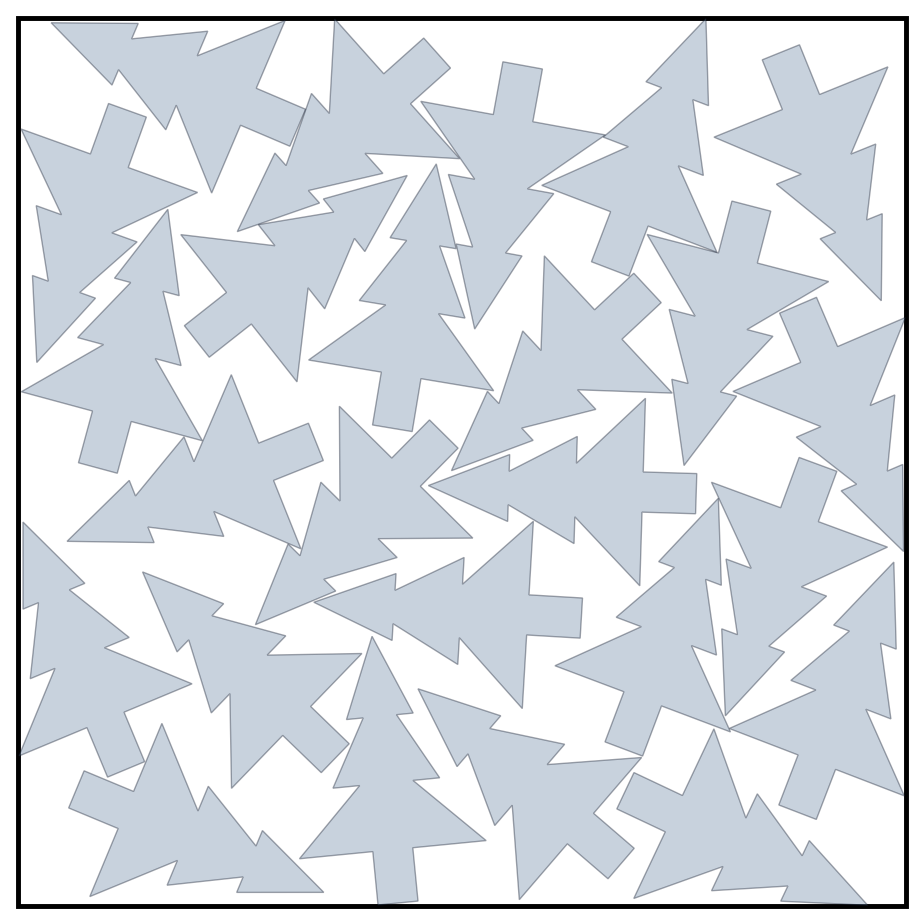
\includegraphics[width=0.32\linewidth]{img/per_n_configs/N025_best_config}\\[0.8em]
  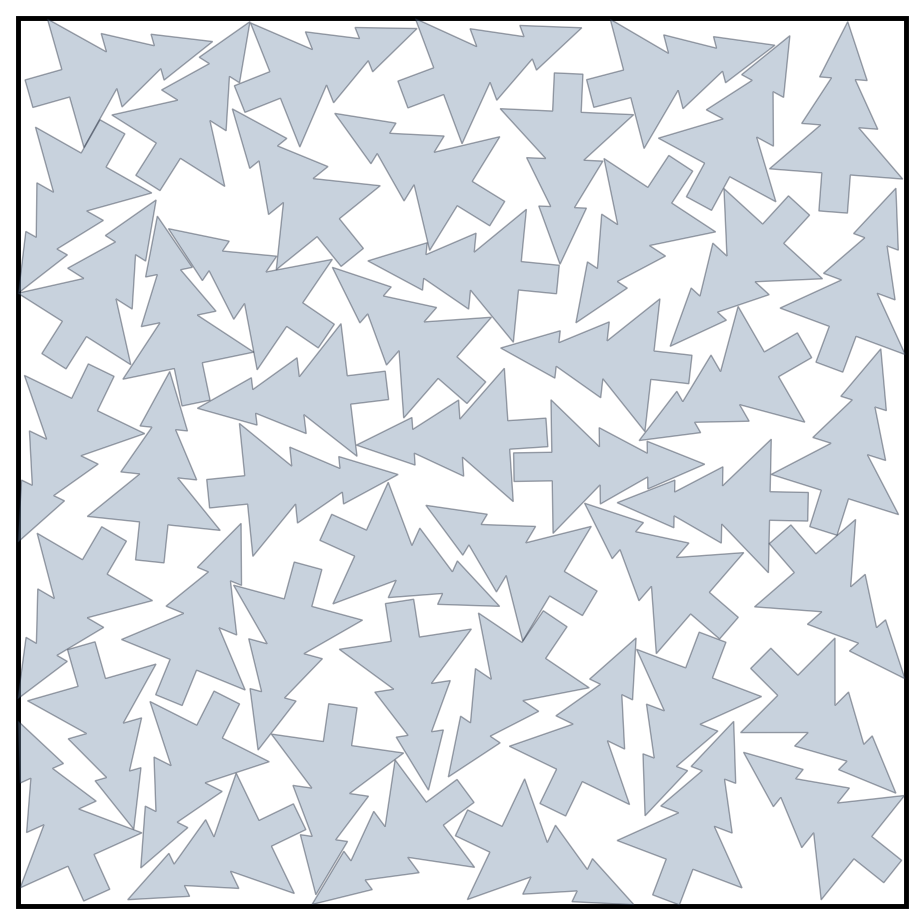
\includegraphics[width=0.32\linewidth]{img/per_n_configs/N050_best_config}\hfill
  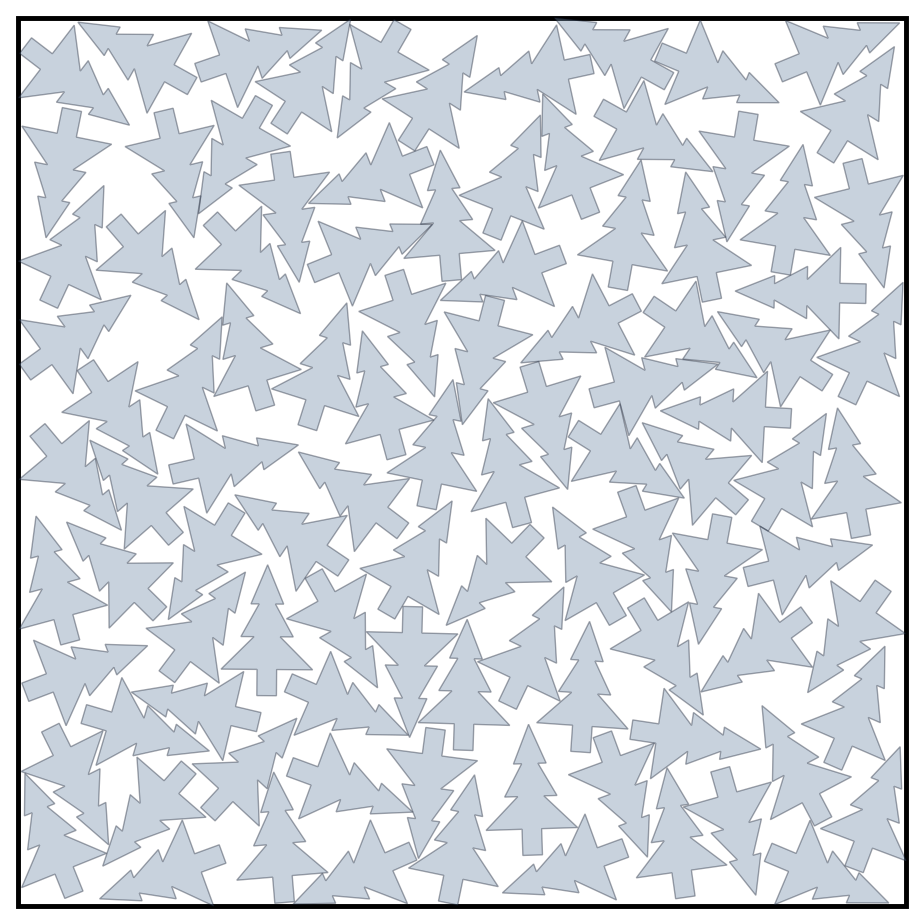
\includegraphics[width=0.32\linewidth]{img/per_n_configs/N100_best_config}\hfill
  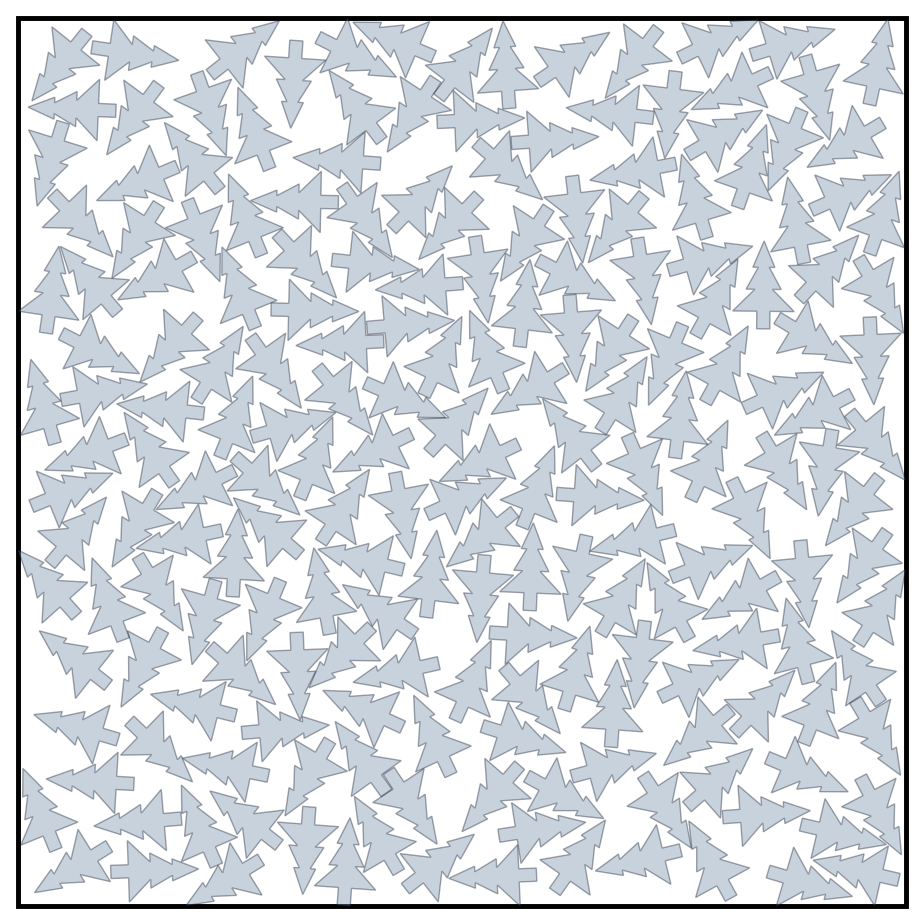
\includegraphics[width=0.32\linewidth]{img/per_n_configs/N200_best_config}
  \caption{Best recovered packing geometries by instance size.
  Top row: $N=5,10,25$. Bottom row: $N=50,100,200$.}
  \label{fig:pernconfigs}
\end{figure*}

Figure~\ref{fig:density} shows the best-so-far packing density
$\eta = NA_p/L^2$ over wall time. Rapid initial improvement reflects
the bisection phase locking in a feasible bracket; the subsequent slow
tail is the adaptive polish making incremental gains. At large $N$
the density gain during polish is proportionally larger, confirming that
the most computationally expensive part of the search is also the most
productive.

\begin{figure}[h]
  \centering
  \includegraphics[width=\columnwidth]%
    {img/feasible_best_density_timeseries}
  \caption{Best-so-far packing efficiency $\eta$ versus wall time.
  Each panel corresponds to one instance size. Thin lines are
  individual worker traces; the black line is the median across
  workers that found feasibility.}
  \label{fig:density}
\end{figure}

Figure~\ref{fig:timetobest} shows the distribution of time to final
best configuration per instance size. At $N=5$ and $N=10$, most workers
converge within a few minutes. At $N=50$ and $N=100$, the interquartile
range spans thousands of seconds, indicating that the polish phase is
essential and that runs benefit from longer wall-time allocations.

\begin{figure}[h]
  \centering
  \includegraphics[width=\columnwidth]%
    {img/feasible_time_to_best_by_n}
  \caption{Distribution of wall time to final best feasible
  configuration by $N$. Boxes show interquartile range; dots are
  individual workers. The dramatic increase at $N \geq 50$ motivates
  longer allocations and more workers at large instance sizes.}
  \label{fig:timetobest}
\end{figure}

\subsection{Density Scaling with $N$}

Figure~\ref{fig:densityscaling} shows packing efficiency $\eta$ as a
function of $N$ (left panel) and as a function of $1/\!\sqrt{N}$ (right
panel), computed from best available runs at
$N=5,10,20,25,50,100,200$. A roughly linear relationship with
$1/\!\sqrt{N}$ suggests that density follows
$\eta(N) \approx \eta_\infty + c/\!\sqrt{N}$ for some constants
$\eta_\infty$ and $c > 0$: as polygons become more numerous, the
achievable density approaches a limiting value from above.

\begin{figure}[h]
  \centering
  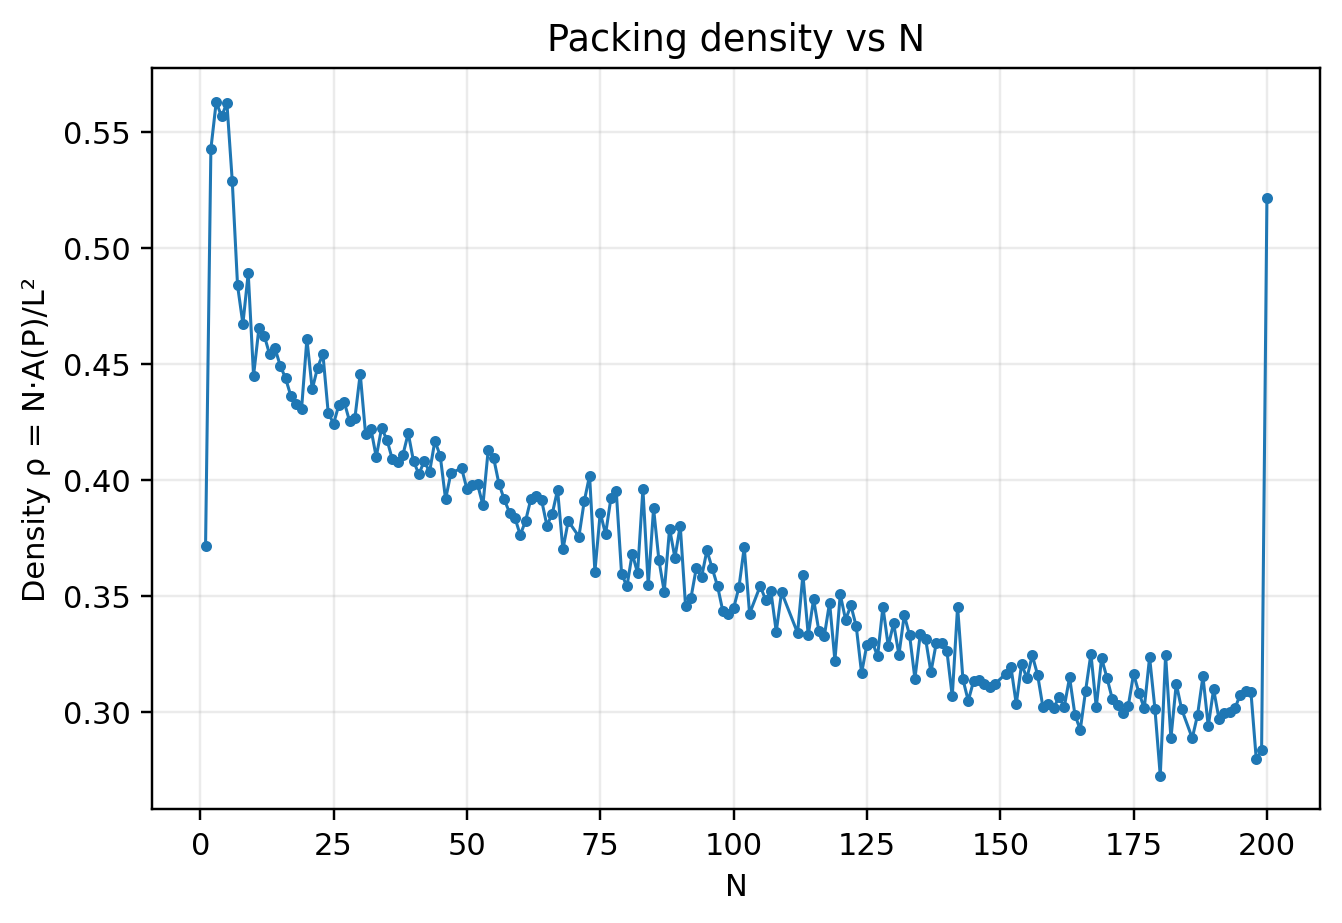
\includegraphics[width=0.485\columnwidth]{img/density_vs_N}%
  \hfill
  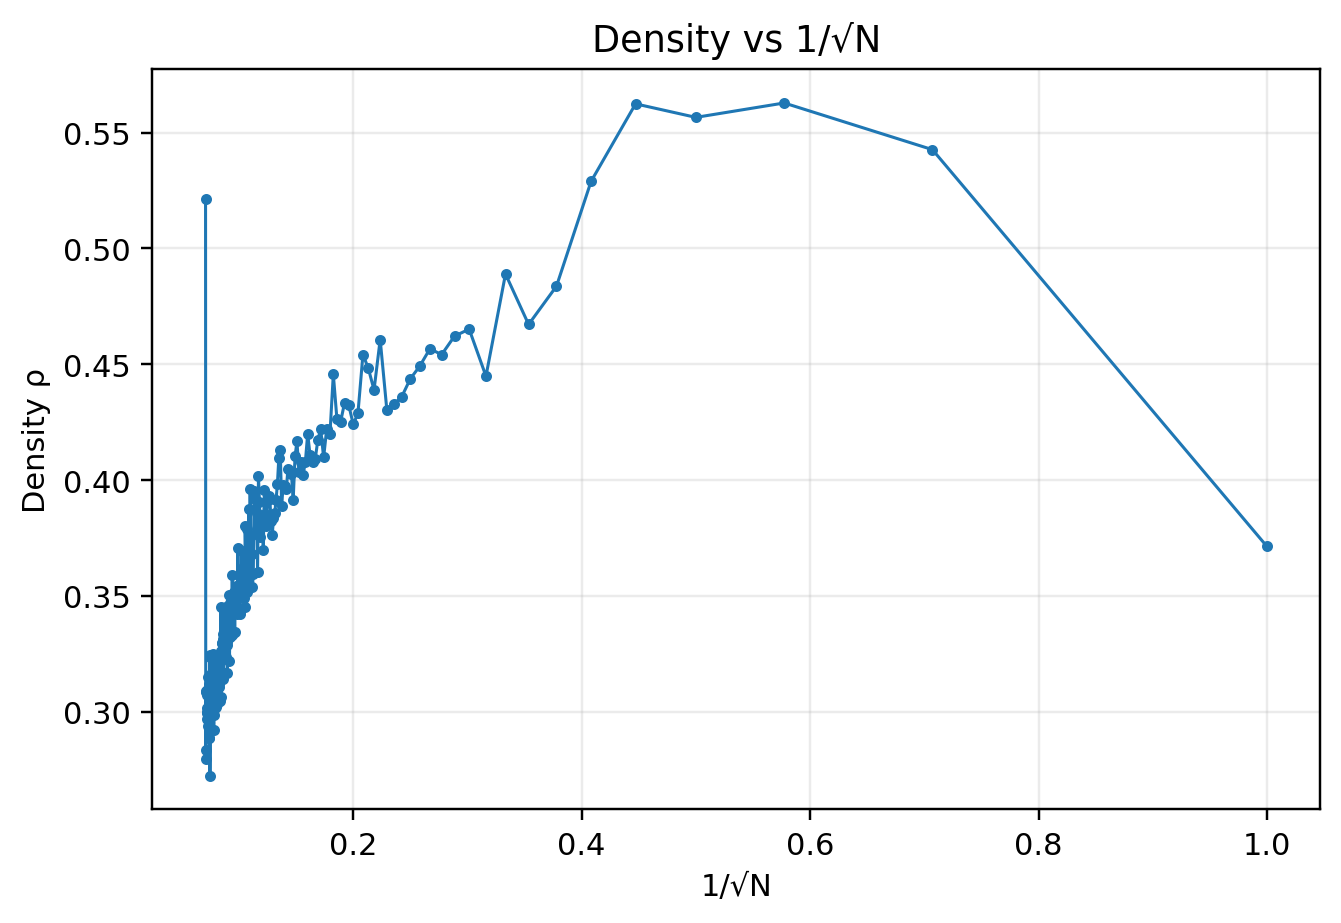
\includegraphics[width=0.485\columnwidth]{img/density_vs_inv_sqrtN}
  \caption{Packing efficiency $\eta$ versus $N$ (left) and versus
  $1/\!\sqrt{N}$ (right). The approximately linear relationship with
  $1/\!\sqrt{N}$ suggests $\eta(N) \approx \eta_\infty + c/\!\sqrt{N}$
  with a limiting density $\eta_\infty$ as $N \to \infty$.}
  \label{fig:densityscaling}
\end{figure}

% ============================================================
\section{Conclusion}
\label{sec:conclusion}

The solver described here combines two-phase SA with an outer
bracketing-bisection loop and an adaptive polish stage. Using SAT
penetration depth rather than a binary overlap test was the choice that
made the energy approach viable: depth provides the continuous gradient
that steers SA toward feasibility from arbitrary initial configurations.
The bracketing-bisection loop certifies $L^*$ to absolute precision
$3.7\times 10^{-9}$ after 26 steps under a 0.25-unit initial bracket,
and the polish phase then uses the remaining wall time productively.

The experiments reveal a clear bottleneck at large $N$: the fixed
iteration budget $M$ is insufficient to adequately explore each polygon's
degrees of freedom when $N \geq 100$, and the fraction of workers
reaching feasibility drops from near-certain at $N \leq 10$ to a single
run at $N = 200$. Scaling $M$ proportionally to $N$, combined with
longer wall times, is the first intervention to try.

\paragraph{GPU acceleration.}
Both the incremental pair-penalty computation and the embarrassingly
parallel multi-trial structure map naturally to GPU architecture. A
CUDA implementation could assign one thread block per polygon pair,
keeping triangle vertex arrays in shared memory and running the SAT
kernel without global memory traffic. The target platform on the
cluster is an NVIDIA Tesla P100 (compute capability 6.0), where memory
bandwidth governs the SAT loop throughput.

\paragraph{Advanced SA variants.}
Elite-Resample Multi-Start (ER-MS) periodically culls the weakest of
$R$ parallel chains and reinitialises them from elite configurations,
concentrating the search near low-energy regions without full
communication overhead. Parallel Tempering (PT) runs $R$ chains at a
geometric temperature ladder and proposes Metropolis swaps between
adjacent temperatures; the swap criterion preserves the joint Gibbs
distribution, and high-temperature replicas can seed cold-chain
refinement with configurations near deep, narrow feasibility basins.
Under the budget tested here, PT found no feasible solutions, but
substantially longer runs may reveal its advantages.

\paragraph{Genetic algorithms.}
A GA treating full layouts as chromosomes and combining them via
crossover could maintain structural diversity across many qualitatively
different configurations simultaneously, something a single SA chain
cannot do. Defining a crossover operator for continuous rigid-body
placements that preserves good partial arrangements (such as a tightly
packed cluster of pieces) is the main technical challenge, and a
controlled GA-versus-SA benchmark on this instance family would be a
productive next experiment.

% ============================================================
\bibliographystyle{plain}
\begin{thebibliography}{10}

\bibitem{kirkpatrick1983}
S.~Kirkpatrick, C.~D. Gelatt, and M.~P. Vecchi.
Optimization by simulated annealing.
\textit{Science}, 220(4598):671--680, 1983.

\bibitem{demaine2007}
E.~D. Demaine and J.~O'Rourke.
\textit{Geometric Folding Algorithms: Linkages, Origami, Polyhedra}.
Cambridge University Press, 2007.

\bibitem{bennell2008}
J.~A. Bennell and J.~F. Oliveira.
The geometry of nesting problems: A tutorial.
\textit{European Journal of Operational Research}, 184(2):397--415, 2008.

\bibitem{ghosh1993}
P.~K. Ghosh.
A unified computational framework for Minkowski operations.
\textit{Computers and Graphics}, 17(4):357--378, 1993.

\bibitem{leung2003}
T.~W. Leung, C.~K. Chan, and M.~D. Troutt.
Application of a mixed simulated annealing-genetic algorithm heuristic
for the two-dimensional orthogonal packing problem.
\textit{European Journal of Operational Research}, 145(3):530--542, 2003.

\bibitem{jakobs1996}
S.~Jakobs.
On genetic algorithms for the packing of polygons.
\textit{European Journal of Operational Research}, 88(1):165--181, 1996.

\bibitem{burke2006}
E.~K. Burke, G.~Kendall, and G.~Whitwell.
A new placement heuristic for the orthogonal stock-cutting problem.
\textit{Operations Research}, 52(4):655--671, 2004.

\bibitem{hukushima1996}
K.~Hukushima and K.~Nemoto.
Exchange Monte Carlo method and application to spin glass simulations.
\textit{Journal of the Physical Society of Japan}, 65(6):1604--1608, 1996.

\bibitem{earl2005}
D.~J. Earl and M.~W. Deem.
Parallel tempering: Theory, applications, and new perspectives.
\textit{Physical Chemistry Chemical Physics}, 7:3910--3916, 2005.

\bibitem{Hajek1988}
B.~Haj\'ek.
Cooling schedules for optimal annealing.
\textit{Mathematics of Operations Research}, 13(2):311--329, 1988.

\end{thebibliography}

\end{document}